\UseRawInputEncoding
\documentclass{beamer}
\usepackage[utf8]{inputenc}

\usetheme{Madrid}
\usecolortheme{default}
\usepackage{amsmath,amssymb,amsfonts,amsthm}
\usepackage{txfonts}
\usepackage{tkz-euclide}
\usepackage{listings}
\usepackage{adjustbox}
\usepackage{array}
\usepackage{tabularx}
\usepackage{gvv}
\usepackage{lmodern}
\usepackage{circuitikz}
\usepackage{tikz}
\usepackage{graphicx}

\lstset{
  literate={≠}{{$\neq$}}1 {→}{{$\to$}}1
}

\setbeamertemplate{page number in head/foot}[totalframenumber]

\usepackage{tcolorbox}
\tcbuselibrary{minted,breakable,xparse,skins}



\definecolor{bg}{gray}{0.95}
\DeclareTCBListing{mintedbox}{O{}m!O{}}{%
  breakable=true,
  listing engine=minted,
  listing only,
  minted language=#2,
  minted style=default,
  minted options={%
    linenos,
    gobble=0,
    breaklines=true,
    breakafter=,,
    fontsize=\small,
    numbersep=8pt,
    #1},
  boxsep=0pt,
  left skip=0pt,
  right skip=0pt,
  left=25pt,
  right=0pt,
  top=3pt,
  bottom=3pt,
  arc=5pt,
  leftrule=0pt,
  rightrule=0pt,
  bottomrule=2pt,
  toprule=2pt,
  colback=bg,
  colframe=orange!70,
  enhanced,
  overlay={%
    \begin{tcbclipinterior}
    \fill[orange!20!white] (frame.south west) rectangle ([xshift=20pt]frame.north west);
    \end{tcbclipinterior}},
  #3,
}
\lstset{
    language=C,
    basicstyle=\ttfamily\small,
    keywordstyle=\color{blue},
    stringstyle=\color{orange},
    commentstyle=\color{green!60!black},
    numbers=left,
    numberstyle=\tiny\color{gray},
    breaklines=true,
    showstringspaces=false,
}
%------------------------------------------------------------
%This block of code defines the information to appear in the
%Title page
\title %optional
{2.6.22}
%\subtitle{A short story}

\author % (optional)
{AI25BTECH11013-Gautham}


\begin{document}


\frame{\titlepage}
\begin{frame}{Question}
Given vectors $\Vec{a} = 2\overrightarrow{i} + \overrightarrow{j} + 3\overrightarrow{k}$ and $\Vec{b} = 3\overrightarrow{i} + 5\overrightarrow{j} - 2\overrightarrow{k}$, find $|\Vec{a} \times \Vec{b}|$.\\
\end{frame}

\begin{frame}{Theoretical Solution}
The cross product or vector product of two vectors $\Vec{A} = \myvec{A_{1} \\ A_{2} \\ A_{3}}$ and $\Vec{B} = \myvec{B_{1} \\ B_{2} \\ B_{3}}$ is defined as:
\begin{align}
\Vec{A} \times \Vec{B} = \myvec{
A_{2} B_{3} - A_{3} B_{2}\\
A_{3} B_{1} - A_{1} B_{3} \\
A_{1} B_{2} - A_{2} B_{1}
}
\end{align}

Now, given
\begin{align}
\Vec{a} &= \myvec{2 \\ 1 \\ 3}, \quad
\Vec{b} = \myvec{3 \\ 5 \\ -2}
\end{align}
\end{frame}

\begin{frame}{Theoretical Solution}
Using the formula for cross product,
\begin{align}
\Vec{a} \times \Vec{b} &= \myvec{
1 \times (-2) - 3 \times 5 \\
3 \times 3 - 2 \times (-2) \\
2 \times 5 - 1 \times 3
} \\
&= \myvec{
-2 - 15 \\
9 + 4 \\
10 - 3
} \\
&= \myvec{-17 \\ 13 \\ 7}
\end{align}

Finally, the magnitude of the cross product is:
\begin{align}
||\Vec{a} \times \Vec{b}||&= \sqrt{(-17)^2 + 13^2 + 7^2} \\
&= \sqrt{289 + 169 + 49} \\
&= \sqrt{507}
\end{align}
\end{frame}


\begin{frame}[fragile]
    \frametitle{C Code}

    \begin{lstlisting}
#include <stdio.h>

void crossProduct(int a[3], int b[3], int result[3]) {
    result[0] = a[1]*b[2] - a[2]*b[1];
    result[1] = a[2]*b[0] - a[0]*b[2];
    result[2] = a[0]*b[1] - a[1]*b[0];
}
    \end{lstlisting}
\end{frame}

\begin{frame}[fragile]
    \frametitle{C-Python Code}

    \begin{lstlisting}
import numpy as np
import matplotlib.pyplot as plt
import ctypes
import numpy.linalg as linalg
from mpl_toolkits.mplot3d import Axes3D
lib = ctypes.CDLL('./func.so')

lib.crossProduct.argtypes = [
    ctypes.POINTER(ctypes.c_int),  
    ctypes.POINTER(ctypes.c_int),  
    ctypes.POINTER(ctypes.c_int)   
]
lib.crossProduct.restype = None
    \end{lstlisting}
\end{frame}

\begin{frame}[fragile]
    \frametitle{C-Python Code}

    \begin{lstlisting}
A = (ctypes.c_int * 3)(2, 1, 3)
B = (ctypes.c_int * 3)(3, 5, -2)
C = (ctypes.c_int * 3)()
lib.crossProduct(A,B,C)
normC=linalg.norm(C)
print(normC)
fig=plt.figure()
ax = fig.add_subplot(111, projection='3d') 
O= [0, 0, 0] 
ax.quiver(*O, *A, color='r', label='a', linewidth=2) 
ax.quiver(*O, *B, color='g', label='b', linewidth=2)
ax.quiver(*O, *C, color='b', label='a * b', linewidth=2)
    \end{lstlisting}
\end{frame}

\begin{frame}[fragile]
    \frametitle{C-Python Code}
    \begin{lstlisting}
ax.text(A[0], A[1], A[2], 'a', color='r', fontsize=12)
ax.text(B[0], B[1], B[2], 'b', color='g', fontsize=12)
ax.text(C[0], C[1], C[2], 'a * b', color='b', fontsize=12)
ax.set_xlabel('X')
ax.set_ylabel('Y')
ax.set_zlabel('Z')
ax.set_xlim([-20,5]) 
ax.set_ylim([0,15])
ax.set_zlim([-5,10])
ax.set_title('plotting a,b,a*b')
plt.savefig("/home/gauthamp/ee1030-2025/ai25btech11013/matgeo/2.6.22/figs/plotc.png")
plt.show()
    \end{lstlisting}
\end{frame}

\begin{frame}[fragile]
    \frametitle{Python Code}
    \begin{lstlisting}
import numpy as np
import numpy.linalg as linalg
import matplotlib.pyplot as plt
from mpl_toolkits.mplot3d import Axes3D
A=np.array([2,1,3])
B=np.array([3,5,-2])
C=np.cross(A,B)
normC=linalg.norm(C)
fig=plt.figure()
ax = fig.add_subplot(111, projection='3d') 
O= [0, 0, 0] 
ax.quiver(*O, *A, color='r', label='a', linewidth=2) 
ax.quiver(*O, *B, color='g', label='b', linewidth=2)
ax.quiver(*O, *C, color='b', label='a * b', linewidth=2)
    \end{lstlisting}
\end{frame}

\begin{frame}[fragile]
    \frametitle{Python Code}
    \begin{lstlisting}
ax.text(A[0], A[1], A[2], 'a', color='r', fontsize=12)
ax.text(B[0], B[1], B[2], 'b', color='g', fontsize=12)
ax.text(C[0], C[1], C[2], 'a * b', color='b', fontsize=12)
ax.set_xlabel('X')
ax.set_ylabel('Y')
ax.set_zlabel('Z')
ax.set_xlim([-20,5]) 
ax.set_ylim([0,15])
ax.set_zlim([-5,10])
ax.set_title('plotting a,b,a*b')
plt.savefig("/home/gauthamp/ee1030-2025/ai25btech11013/matgeo/2.6.22/figs/plot.png")
plt.show()
    \end{lstlisting}
\end{frame}

\begin{frame}{Plot}
    \centering
    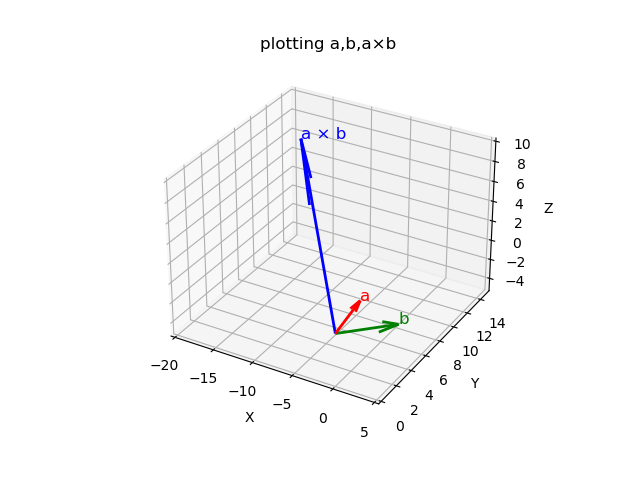
\includegraphics[width=\columnwidth, height=0.8\textheight, keepaspectratio]{figs/plot.png}     
\end{frame}
\end{document}
